w\documentclass[11pt, oneside]{article}
\usepackage[english]{babel}
\usepackage[T1]{fontenc}
\usepackage[utf8x]{inputenc}
\usepackage{amsmath}
\usepackage{graphicx}
\usepackage{microtype}
\usepackage{float}
\usepackage{epstopdf}
\usepackage{datetime}
\usepackage[super]{nth}
%\usepackage{subfigure}
\usepackage{caption}
\usepackage{subcaption}
\usepackage[left=3.5cm, right=3cm, top=3cm, bottom=3cm]{geometry}
\usepackage{wrapfig}
\usepackage{lipsum}
\usepackage{booktabs}
\usepackage{siunitx}
\usepackage{listings}
\usepackage[svgnames]{xcolor}
\usepackage{cite}

\definecolor{ciao}{RGB}{240,240,240}
\lstset{language=R,
    basicstyle=\small\ttfamily,
    stringstyle=\color{DarkGreen},
    otherkeywords={0,1,2,3,4,5,6,7,8,9},
    morekeywords={TRUE,FALSE},
    tabsize=2,
    backgroundcolor = \color{ciao},
    breaklines=true,
    deletekeywords={data,frame,length,as,character},
    keywordstyle=\color{blue},
    commentstyle=\color{DarkGreen},
}

\DeclareMathOperator*{\argmax}{arg\,max}
\DeclareMathOperator*{\argmin}{arg\,min}
\DeclareMathOperator{\silhouette}{sil}

\begin{document}

\begin{titlepage}


\center

\textsc{\Large Sant'Anna School of Advanced Studies}\\[1.5cm]

\includegraphics[scale=.3]{sssup.eps}\\[1.5cm]
\textsc{\LARGE Topics in Statistical Learning}\\[0.7cm]
\Large{Prof. Francesca \textsc{Chiaromonte}}\\[1.6cm]

{ \huge{\textsc{Cutting through the Vibes}}}\\[0.2cm]
{ \huge{\textsc{Sound-Frequency Data}}}\\[0.2cm]
{ \huge{\textsc{Across Musical Genres}}}\\[3.6cm]


\begin{flushleft} \Large
\emph{Authors:}\\
Alfredo \textsc{Bochicchio}\\
Corrado \textsc{Calemma}\\
Leonardo \textsc{Lai}\\
Emanuele \textsc{Orsini}\\
\end{flushleft}

\large{March \nth{28}, 2019}\\[2cm] 
\vfill 

\end{titlepage}
\newpage
\pagenumbering{roman}
\section*{\textsc{Abstract}}
For the sake of track recognition, building and tuning recommendation engines for well-known end-user streaming services, and many other goals, musical tracks have lately become the object of an ever broader spectrum of statistical analysis procedures aimed at finding efficient ways to distinguish and classify every single instance of musical expression. Following this growing interest, a remarkable number of datasets concerning huge quantities of tracks currently available on mainstream commercial platforms has been made accessible to the public. While most of them are focused on metadata that disregard the perceptual characteristics of tracks, some include also many variables representing key sound-frequency features. The following essay is meant to offer a rudimentary glimpse of how the data contained in the latter ones can be smoothly (and successfully) used $-$ performing respectively a series of supervised and unsupervised analysis techniques on a dataset that stands out for the number of perception-relating variables $-$ both to show regularities within and across genres, and to help perform genre classification for previously unclassified tracks.
\vspace{0.5cm}
\tableofcontents
\newpage
\pagenumbering{arabic}
\section[Introduction]{\textsc{Introduction}}
Over the last couple of decades, consumers have been able to witness the rise of a large number of commercial services making huge amounts of music immediately available for them to purchase or even directly listen. Immense catalogues of music tracks became immediately accessible (for the sheer sake of indicating the order of magnitude, iTunes store opened in 2003 with an offer of 200.000 songs, just to end up in 2017 offering over 40 million tracks alongside the streaming service Apple music; Spotify currently operates around similar numbers, with an estimated 35 million tracks as of 2018). It was just a matter of time before it became evident that users could enjoy some tools allowing them not to get lost in their experience of these enormous repositories. Mechanisms suggesting songs similar to those users already listen to from a stylistic and perceptual point of view, or even some that are, at least apparently, more ambitious, like Shazam or SoundHound, allowing users with a mobile handset to obtain the name of the track they are hearing in their surrounding environment.

It is obvious that anyone willing to create or even to tune the inner workings of these tools needs very large datasets of songs from which to extract information concerning the perceptual properties of single tracks, or even some physical features of the sound frequencies recorded and then reproduced for end users. Currently, even if most of them are exclusively accessible to those who work for the music industry, a few of them have been made publicly available. One of the most remarkable public dataset to date -- both for its extensions and for the amount of information it offers in terms of the number of tracks considered -- is the FMA dataset, which contains both raw tracks and sound-frequency data computed from them.

The primary aim of this paper is clearly not to show how these devices use these data to work, but offer a glimpse how this kind of data can provide us with precious information even without recurring to esoteric, extremely sophisticated data analysis methods. This is done performing a series of statistical analysis techniques (using R as our software choice) on the sound-frequency process data provided by the FMA dataset.


The work will be divided into two main parts, according to the the nature of the procedures that have been reported and commented: the first part will contain the accounts of unsupervised procedures, originally performed in order to bring to light any possible regularity within and across single musical genres. More specifically, this part will cover the results that have been obtained by trying to clusterize tracks observations from single genres and to perform principal component analysis. The second part will expose some attempts at genre classification (namely by Linear and Quadratic Discriminant Analysis, along with k Nearest Neighbors classification), carried out in order to ascertain whether the data at our disposal can be effectively and efficiently used to classify songs by genre.

As the pages that follow will report more accurately, some of the results obtained were satisfyingly surprising: as a matter of fact, while the supervised analysis results estimates showed simple but clear regularities across genres, the supervised analysis techniques we used to try to classify the tracks by genres showed that the most effective procedures were also the simplest ones (although by a small margin).

\newpage

\section[The dataset]{\textsc{The dataset}}
\subsection{Some theoretical considerations}

Free Music Archive is an open and easily accessible dataset built for research purposes. It provides full length and high quality audio, pre computed features, together with track and user level metadata, tags, and free form text such as biographies. This impressive dataset derives from the elaboration of 917 GB of raw audio data, 343 days of total audio length, divided in 106.574 tracks from more than 16.000 artists and 161 different genres in total. We use only a small subset of the available data for the sake of computation and ease of use.

The Free Music Archive is the first real attempt to provide an open source database with pre-computed features which enables researchers who do not dispose of sufficient computational resources to do some exstensive data analysis. Many resources are already avaiable in image and video analysis, and convolutional neural networks have been around for more than a decade now. FMA would like to become the musical equivalent of the well known MINST dataset for number and character recognition. 

\begin{wraptable}{r}{6.2cm}
\begin{tabular}{lc}
\hline
 & dimension \\ \hline
1 Chroma & 84 \\
2 Tonnetz & 42 \\
3 MFCC & 140 \\
4 Spectral Centroid & 7 \\
5 Spectral Bandwidth & 7 \\
6 Spectral Contrast & 49 \\
7 Spectral Rolloff & 7 \\
8 RMS Energy & 7 \\
9 Zero-crossing Rate & 7 \\ \hline
\end{tabular}
\caption{Precomputed features list}
\label{my-label}
\end{wraptable}

Variables concerning every single class of features are pre-computed by taking seven statistics over a sample period, corresponding to 1.5 seconds of the song. The statistics are the following: mean, standard deviation, skewness, kurtosis, median, minimum, and maximum value.

It is important to notice that we often identified smaller sub-samples of the dataset in order to provide more reasonable results in both supervised and unsupervised contexts. The chosen subset is strongly dependent on the tasks we set out to do. Specifically, we selected only the most representative genres and within the genres, we only based our analysis on Chroma features, Tonnetz and MFCC, confronting what seemed to be the most meaningful statistics: mean and skewness.
\begin{figure}[h]
    \centering
    \begin{subfigure}[b]{0.30\textwidth}
        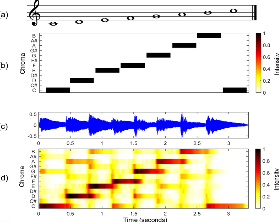
\includegraphics[width=\textwidth]{b.png} 
        \caption{Chroma Features}
        \label{fig:RBFgamma}
    \end{subfigure}\hfill
    \begin{subfigure}[b]{0.30\textwidth}
        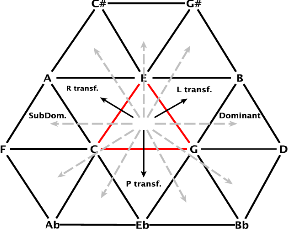
\includegraphics[width=\textwidth]{c.png}
        \caption{Tonnetz}
        \label{fig:RBFgamma2}
    \end{subfigure}\hfill
    \begin{subfigure}[b]{0.30\textwidth}
        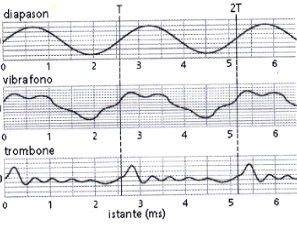
\includegraphics[width=\textwidth]{d.png}
        \caption{Timbre}
        \label{fig:RBFgamma3}
    \end{subfigure}
    \caption{Features}
    \label{fig:svmrbfC}
\end{figure}

\begin{itemize}
    \item \emph{Chroma features}: relates to the 12 different pitch classes. Fourier Spectral Decomposition of a sample gives the intensity at a given frequency.
    \item \emph{Tonnetz, Tonalities}: conceptual lattice diagram representing the tonal space. They describe the single notes played within the samples.
    \item \emph{MFCC}, \emph{Mel Frequency Cepstrum} or \emph{Timbre}: it distinguishes different types of sound production, such as choir voices and musical instruments. It represents the distribution of the frequencies in the fourier series.
    In order to obtain MFCC: take the Fourier transform of (a windowed excerpt of) a signal, map the powers of the spectrum obtained above onto the mel scale, take the logs of the powers at each of the Mel frequencies.
    MFCC values are not very robust in the presence of additive noise, so they had to be normalized.
\end{itemize}

\subsection{Data selection and pre-processing}
As the previous paragraphs have explained, the dataset provides a considerable wealth of information for a remarkable number of musical tracks, making it consequently possible to choose among a vast number of alternatives, both from the point of view of the analyses that can be performed on the data, and from the point of view of the variables that can be considered for the purposes of these same analyses. This consideration has both technical and statistical implications. From a more technical perspective, as already mentioned, the precomputed-features dataset characterizes its observations with variables that capture different aspects of the 1.5 seconds sample associated to each one of the tracks, each one behaving in potentially different ways within or across musical genres. Chroma features, for example, capture the tonal characteristic such as pitch and chords, and there is no reason to believe that they shouldn't show a considerable heterogeneity within musical genres, but we equally had no reason to believe that some pitches could be heavily concentrated within single genres or groups of genres. This line of reasoning inspired our decision to use variables concerning chroma features only  for the unsupervised learning techniques we followed within single musical genres -- in order to see if there was any regularity in the use of pitches that we could somehow get a glimpse of by means of the data we had. Unsure about their possible usefulness in helping us classify songs by musical genres (by means of discriminant analysis or k-nearest neighbors classification), we decided not to use them in the supervised part of our work.

Timbre features involve a completely different kind of information: in this case the pitches or the tonal characteristics of sound are not considered. The only element that matters is the way those sounds are physically generated (although “physically” is just inappropriate as a term, since the dataset in made also of a large number of electronic music tracks, in which sound frequencies are mostly created or edited digitally). This aspect does not allow us to expect a great deal of heterogeneity within single musical genres, but can be useful in distinguishing between them. To put it in extremely simple terms, there are reasons to believe that every mainstream musical genre is associated with a more or less precisely defined set of instruments that sets it apart from other genres; just to make a simple example, no one is used to hearing an electric guitar in a classical track or a synthesizer in a folk song. Since the presence of a specific instrument is presumably captured by timbre features, they make a suitable object of analysis to help us classify songs by genre.

The other aspect of the matter, as we already mentioned in the first paragraph, has a more statistical flavor. Every single variable (including the twelve chroma features and the twenty timbre features) could be measured at every instant of the song. Calculating them at every point of the 1.5 sample does not leave us only with average values, but with full-fledged sample probability distributions, from which the dataset's creators extracted the seven previously mentioned statistics.

The unsupervised techniques we wanted to take advantage of (more specifically clustering) can be highly sensitive to useless variables: highly-informative features allowing us to reach a clearer cluster configuration can be overshadowed by the disturbancies brought by variables which hold no information at all, modifying the distance structure and consequently compromising the outcome of the clustering algorithm as a whole. In this case, variables like maximum and minimum values could easily be discarded, along with kurtosis, median (a bit redundant, given the dataset includes also the mean) and also standard deviation, leaving us only with means and skewnesses.

As for our classification experiments, the feature-selection approach was slightly more data-driven: we started using only the mean values only to try to add second, third and fourth moments of the features’ distributions. Since we weren't able to see any substantial performance improvement, we kept only the mean values.

Once the variables had been selected, a simple look at how genres were distributed within the dataset revealed that many (too many) songs had not a genre lable attached to them, and also that many (still too many) of the 161 genres considered were just too underrepresented for us to be able to extract some significant information. Thus, we decided to select only songs from four among the most represented genres in the dataset -- electronic, folk and rock music, plus classical music for the parts of our work that concern analyzing chroma features, and hip-hop for those regarding analysis on timbre features.

From this point on, the data have undergone two separate kinds of treatment to prepare them for unsupervised and supervised analysis respectively. Data used for clustering and principal component analysis were divided by genre and then (since chroma features means are not invariant to the general loudness of the track) underwent standardization on rows and columns of each data matrix.

For the same reason a row standardization has been performed on the general matrix we used for supervised analysis (although column standardization has been avoided, as we feared it could have biased the estimates of out-of-sample accuracy of our models by cross-validation, as shown better in the next pages).
\newpage
\section[Unsupervised Techniques]{\textsc{Unsupervised Techniques}}
After selecting the data on which we wanted to perform our analyses, we decided that the first part or our work was to be dedicated to see whether single musical genres could hide different clusters according to chroma features data.

\subsection{Cluster Analysis}
The first doubt we encountered was about defining the technical specifications of the clustering algorithms we wanted to use to obtain the stablest and most representative results possible. To get a preview of how the data could be distributed we used the chroma feature matrix of classical tracks, and then tried with a number of versions of the hierarchical clustering algorithm; these were obtained by simply changing the nature of the distance and linkage functions the mechanism relied on.

After seeing that the euclidean distance was the only one allowing us to obtain decent results (i.e. graphs where there were not single clusters aggregating observations one by one up to the top, or graphs that were not so chaotic that we couldn't even figure out a single possible interpretation for the information we found), we focused our attention on selecting a proper linkage function that suited best our needs. The choice was between three canonical options:
\begin{itemize}
    \item The single linkage function, described by $D\left(C_1, C_2\right)= \min_{x_1\in C_1, x_2\in C_2}d\left(x_1, x_2\right)$. A hierarchical clustering algorithm that uses it tends to aggregate elements and clusters in a way that produces long and stringy objects.
    \item The complete linkage function, that can be represented by the expression $D\left(C_1, C_2\right)= \max_{x_1\in C_1, x_2\in C_2}d\left(x_1, x_2\right)$. It produces, unlike single linkage, compact objects, more ball-shaped with respect to the chosen distance function.
    \item The average linkage function, with $D\left(C_1, C_2\right)= \dfrac{1}{\#C_1\#C_2} \sum_{x_1\in C_1, x_2\in C_2}d\left(x_1, x_2\right)$. It tends to produce results that represent a compromise between the two previous alternatives.
\end{itemize}

From a purely theoretical point of view, we already knew that distinctions between chroma feature clusters couldn't be extremely clear and that stringy clusters would have been impossible to interpret. As a matter of fact, pitch classes, if visible through chroma features, distinguish themselves from each other by means of  more pronounced expressions of certain notes on the musical scale. Hence, it is convenient to imagine single clusters concentrated around definite centroids instead of clusters with a more elongated shape.

Coherently with this line of reasoning, our choice fell on the single linkage function coupled with euclidean distance. We were not in the position to make theoretical assumptions concerning the optimal number of clusters to identify, so we relied on elbow plots to get some data-driven suggestions on the best numbers of clusters to partition the datatet into. These plots represent within-cluster sum of squares as a function of the number of clusters identified by a cut to the dendrogram generated by a hierarchical clustering algorithm\footnote{Using $K$ as the number of clusters identified, the total within sum of squares is defined as follows: $W\left(K\right)=\sum_{k=1}^K \sum_{x_i, x_j\in C_k; i\neq j} d^2\left(x_i, x_j\right)$.} (just like the one we have described in the previous paragraph). The optimal number of clusters suggested by this technique is the one after which the total within-cluster sum of squares stops decreasing significantly (indicated by the typical "elbow" in the graph). Elbow plots are shown in Figure \ref{fig:elbplots}.

\begin{figure}[h!]
\centering  
\begin{subfigure}[b]{0.5\textwidth}
        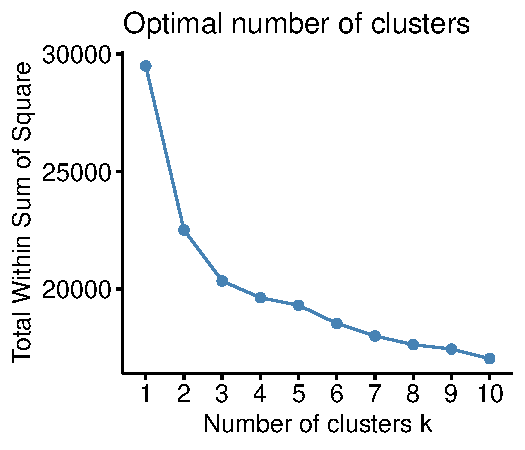
\includegraphics[width=\textwidth]{classic_elbow2.pdf} 
        \caption{Classical}
    \end{subfigure}%
    \begin{subfigure}[b]{0.5\textwidth}
        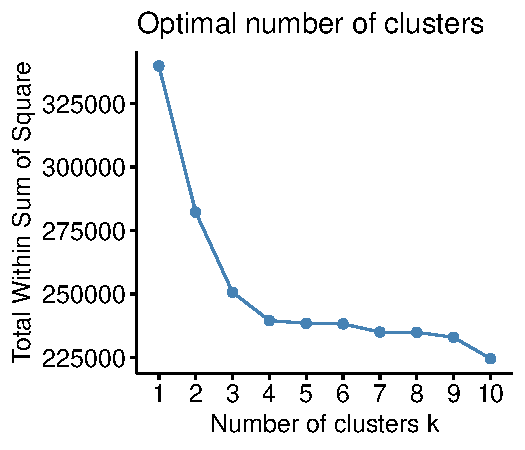
\includegraphics[width=\textwidth]{rock_elbow.pdf} 
        \caption{Rock}
    \end{subfigure} \\
    \vspace{1cm}
    \begin{subfigure}[b]{0.5\textwidth}
        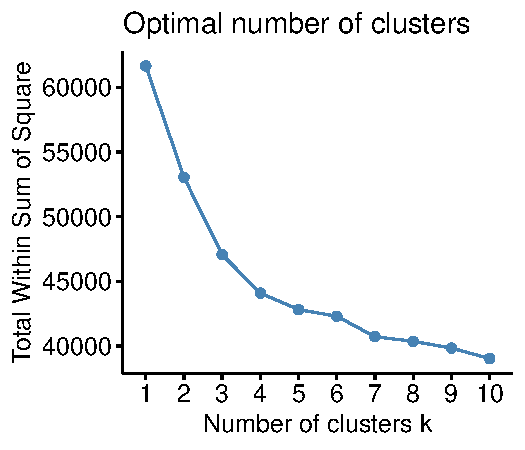
\includegraphics[width=\textwidth]{folk_elbow.pdf} 
        \caption{Folk}
    \end{subfigure}%
    \begin{subfigure}[b]{0.5\textwidth}
        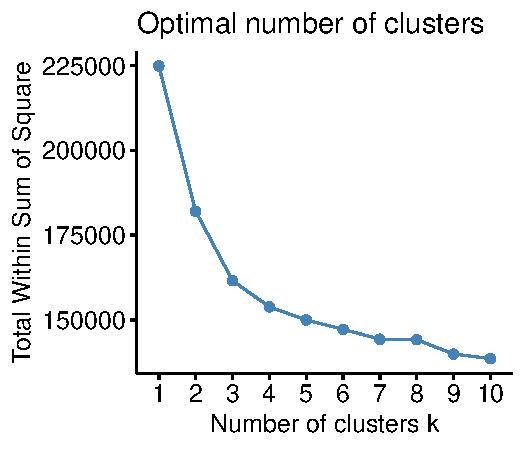
\includegraphics[width=\textwidth]{elec_elbow.pdf} 
        \caption{Electronic}
    \end{subfigure}%
\caption{Hierarchical-kMeans silhouette plots by genre}
\label{fig:elbplots}
\end{figure}


Interestingly enough, the most ambiguous elbow plot we found was the one concerning folk music. In fact, the only interpretation we can give to such results is that a general ambiguity surrounding the possibly optimal number of clusters can be explained by a remarkably variegated use of pitches within the considered genre (in our case, this generates a stark contrast with the stereotypical uniformity of folk as a genre, both from a tonal and from a timbrical point of view).

We are nevertheless aware that the plots in figure \ref{fig:elbplots} don't give us any information concerning the goodness of the results we now have. For this exact reason we chose to look deeper into the matter and to perform some more analyses allowing us to assess the stability of the clustering outcome that our algorithm has produced.

\begin{figure}[h!]
\centering
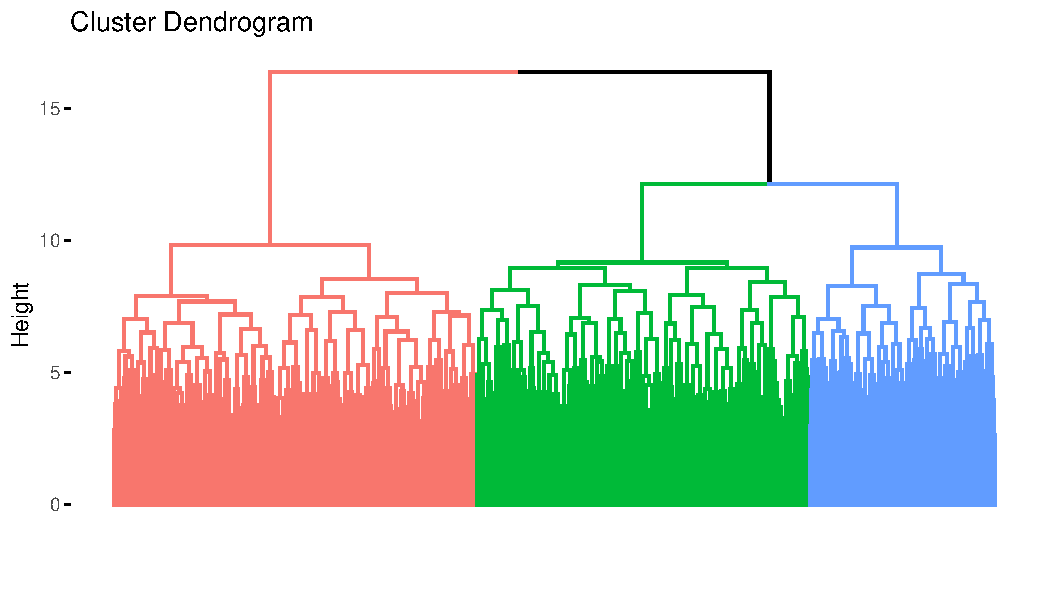
\includegraphics[width=\textwidth]{ciaone_graph.pdf} 
\caption{3-means colorized dendrogram, classical music}
\label{fig:classicdend}
\end{figure}

\begin{figure}[h!]
\centering
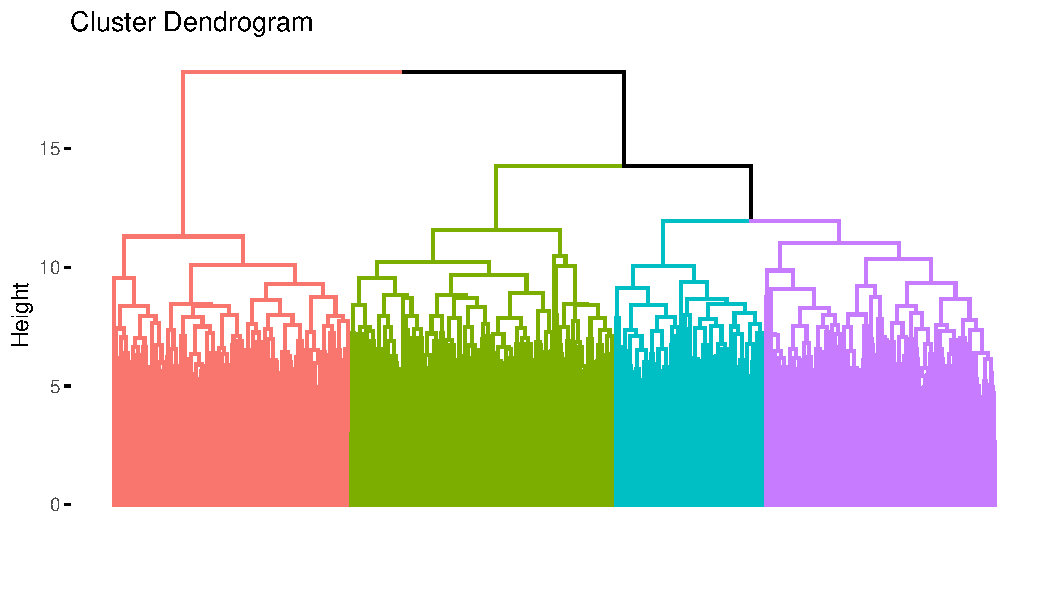
\includegraphics[width=\textwidth]{elec_graph.pdf} 
\caption{4-means colorized dendrogram, electronic music}
\label{fig:elecdend}
\end{figure}
\begin{figure}[h!]
\centering
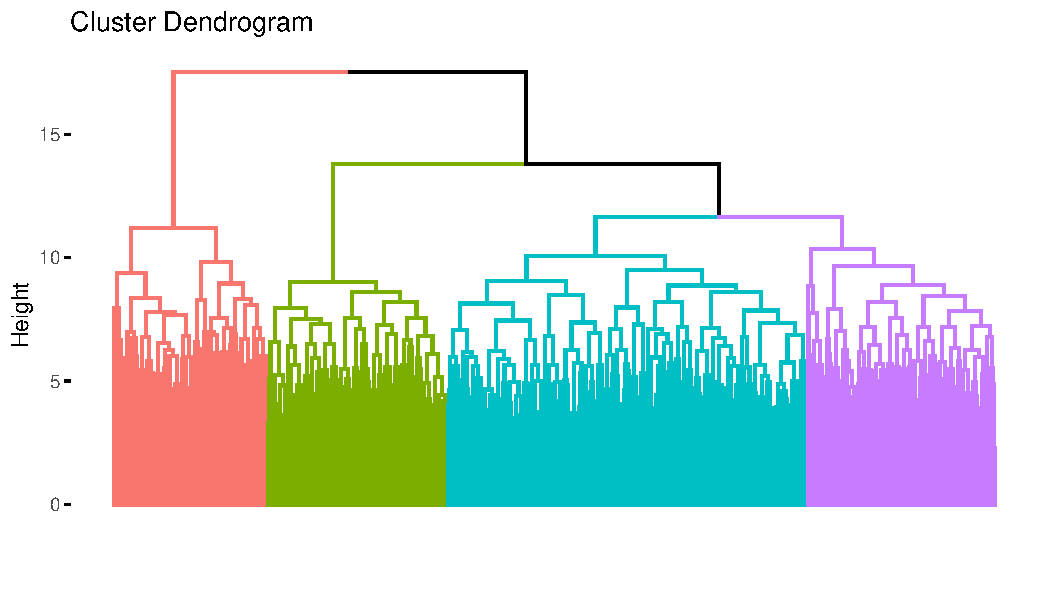
\includegraphics[width=\textwidth]{folk_graph.pdf} 
\caption{4-means colorized dendrogram, folk music}
\label{fig:folkdend}
\end{figure}

\begin{figure}[h!]
\centering
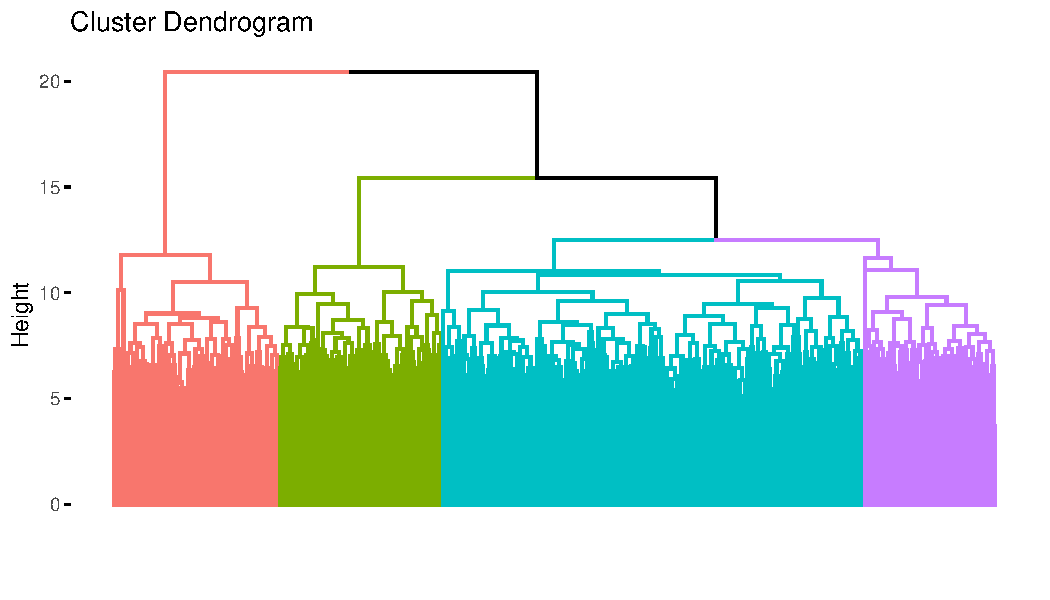
\includegraphics[width=\textwidth]{rock_graph.pdf} 
\caption{4-means colorized dendrogram, rock music}
\label{fig:rockdend}
\end{figure}

One of the techniques that seemed to us extremely suitable for this aim was the hierarchical-k-means clustering algorithm. This procedure extends the simple hierarchical clustering mechanism by extracting the centroids of the clusters produced by it and feeding them to a k-means clustering algorithm. The stability of the clusters identified hierarchically can be assessed by comparing them with the final results of the hybrid algorithm.

By choosing 3 as the optimal number of clusters for classical music, 4 for rock, folk and electronic, we took advantage of a command in R (described in the appendix) colorizing the hierachical clustering dendrograms depending on the outcomes of the hybrid algorithm. Results are shown in Figures \ref{fig:classicdend} to \ref{fig:rockdend}. With striking (and definitely reassuring) regularity, we notice that all the results are extremely stable with respect to the k-means refinement technique we originally decided to use in order to assess the goodness of the clustering outcome.

There is however another sort of ambiguity this kind of information, does not tell us much about how well the clusters are separated from each other, a problem that can be solved by relying on silhouette widths.

\begin{figure}[h]
\centering  
\begin{subfigure}[b]{0.5\textwidth}
        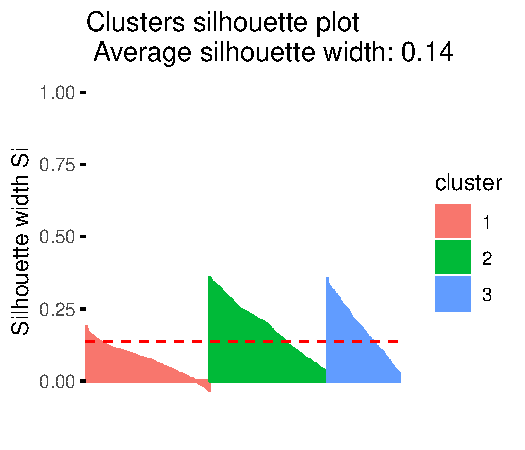
\includegraphics[width=\textwidth]{class_silplot.pdf} 
        \caption{Classical}
    \end{subfigure}%
    \begin{subfigure}[b]{0.5\textwidth}
        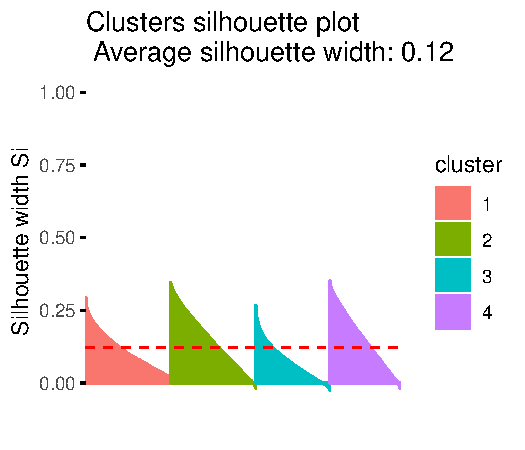
\includegraphics[width=\textwidth]{rock_silplot.pdf} 
        \caption{Rock}
    \end{subfigure} \\
    \begin{subfigure}[b]{0.5\textwidth}
        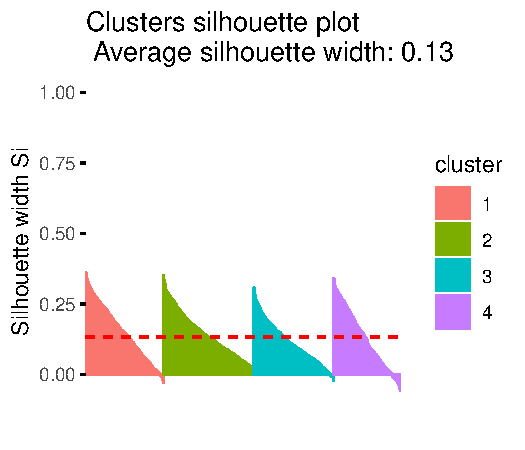
\includegraphics[width=\textwidth]{folk_silplot.pdf} 
        \caption{Folk}
    \end{subfigure}%
    \begin{subfigure}[b]{0.5\textwidth}
        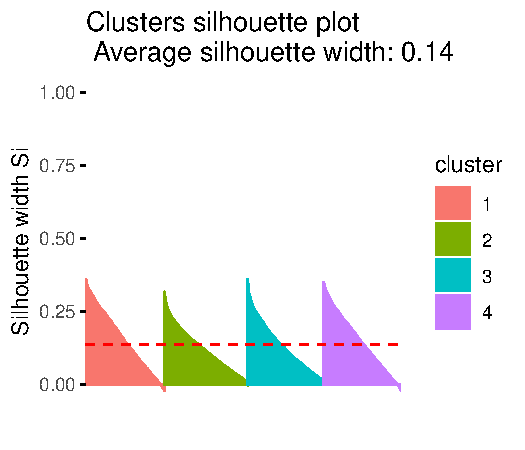
\includegraphics[width=\textwidth]{elec_silplot.pdf} 
        \caption{Electronic}
    \end{subfigure}%
\caption{Hierarchical clustering elbow plots by genre (complete linkage)}
\label{fig:silplots}
\end{figure}

Defining
\[
\delta\left(i,C\right)=\frac{1}{\# C}\sum_{j\in C}d\left(x_i, x_j\right) \quad
\mathrm{and} \quad a_i=\delta\left(i,C\left(i\right)\right), \quad b_i = \min_{C\neq C\left(i\right)} \delta\left(i,C\right)
\]
the silhouette width is expressed as
\[
\silhouette_i = \frac{b_i - a_i}{\max\left\{a_i, b_i\right\}}.
\]


Well-known R packages and commands allow to compute silhouette widths for every single point in a dataset upon which a cluster structure has been imposed. Naturally, observations which have a low value of $a_i$ compared to $b_i$ (and therefore have values of $\silhouette_i$ close to \num{1}) can be considered well clustered; objects for which $a_i$ and $b_i$ have similar values (giving $\silhouette_i$ a value close to \num{0}) are ambiguously positioned, while those for which $a_i > b_i$ (and therefore $\silhouette_i <0$) can be considered to be placed in a wrong cluster (according to the distance used for the evaluation). Results are shown in Figure \ref{fig:silplots}.

As those plots clearly show, the clusters identified by our algorithms are not clearly separated from each other: really low average values and large portions of elements within every single cluster with a silhouette width very close to zero (or even negative in a few cases) certainly do not suggest a tidy cluster structure with a big majority of points lying close to members of the cluster they belong to and much further from members of other clusters. What the silhouette plots suggest is instead a situation in which the regions between clusters hold a considerably high number of points, introducing a margin of uncertainty concerning the correct classification of a significant portion of the total number of observations in each of the four data matrices.
\newpage
\subsection{Principal Component Analysis}
The regularity of the results we obtained by clustering chroma features observations pushed us to analyse the same data from a different point of view. Principal Component Analysis was the technique we chose to extend our work because of the information it can provide about possible links between different variables’ levels of expression, and because of the clarity with which final results can be presented.

By performing the Eigen decomposition of the sample variance-covariance matrix $S=X'X$, with each feature of the dataset centered at 0, PCA allows us to identify the directions (now called Principal Components) within the feature space that are able to capture the biggest fraction of the total variability among observation. This fraction is computed as the ratio between the eigenvalue associated with a specific principal component and the sum of all Eigenvalues obtained by the spectral decomposition).

\begin{figure}[h]
\centering  
\begin{subfigure}[b]{0.5\textwidth}
        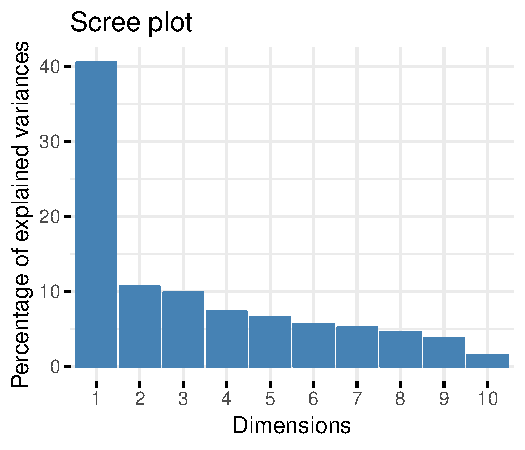
\includegraphics[width=\textwidth]{class_scree.pdf} 
        \caption{Classical}
    \end{subfigure}%
    \begin{subfigure}[b]{0.5\textwidth}
        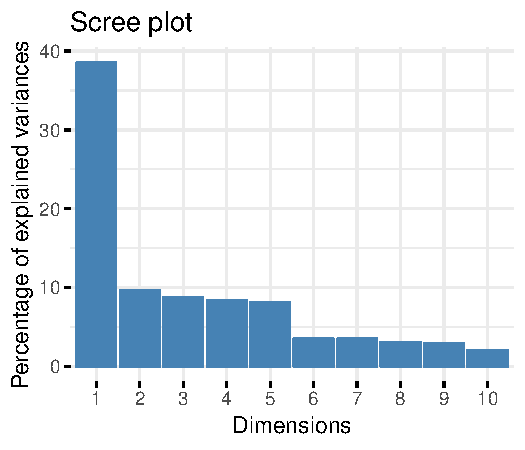
\includegraphics[width=\textwidth]{rock_scree.pdf} 
        \caption{Rock}
    \end{subfigure} \\
    \begin{subfigure}[b]{0.5\textwidth}
        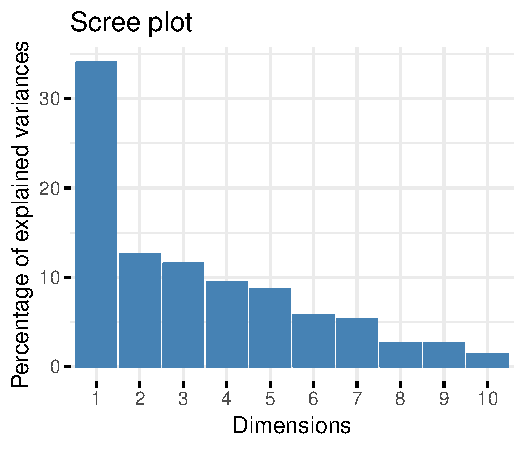
\includegraphics[width=\textwidth]{folk_scree.pdf} 
        \caption{Folk}
    \end{subfigure}%
    \begin{subfigure}[b]{0.5\textwidth}
        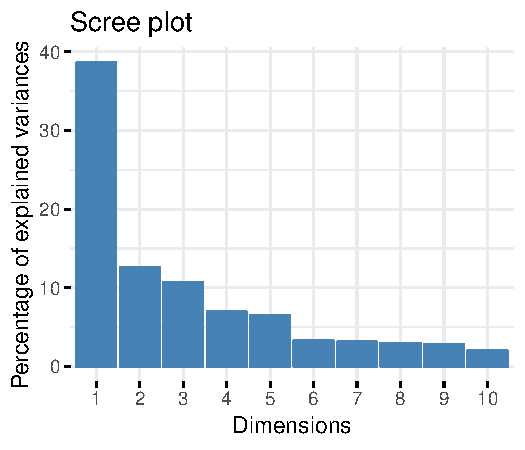
\includegraphics[width=\textwidth]{elec_scree.pdf} 
        \caption{Electronic}
    \end{subfigure}%
\caption{Scree Plots (10 most significant PC's) by genre}
\label{fig:scree}
\end{figure}

Plots showing these ratios for the 10 components associated with the biggest eigenvalues (scree plots) are shown in figure \ref{fig:scree}. Surprisingly enough, if we sought a suggestion concerning the optimal number of PC's to consider from the elbows shown by the scree plots, we should stop at one principal component in each case, as a single eigenvector is able to capture (by a large margin) a significant fraction of the variability within the data.

Interestingly, a simple look at the loadings (the parameters that lie beneath the generation of the principal components as a linear combination of original features) allowed us to see that the first eigenvector in each genre spawns from a linear combination in which the skewnesses have absolutely no role at all (they always start appearing from the second PC on, while the first is dominated by the chroma feature means). Even more interestingly, those first principal components showed similar loadings for all chroma means.

\begin{figure}[h]
\centering  
\begin{subfigure}[b]{0.5\textwidth}
        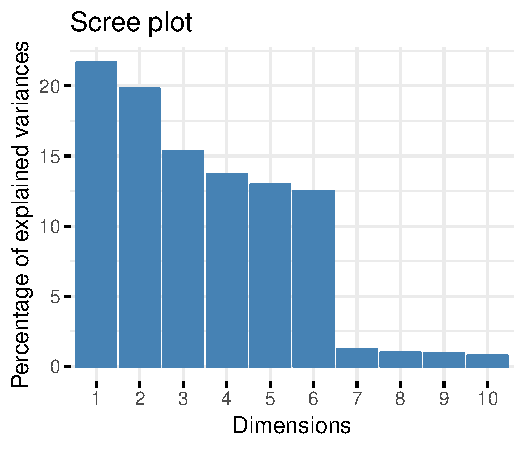
\includegraphics[width=\textwidth]{class_scree2.pdf} 
        \caption{Classical}
    \end{subfigure}%
    \begin{subfigure}[b]{0.5\textwidth}
        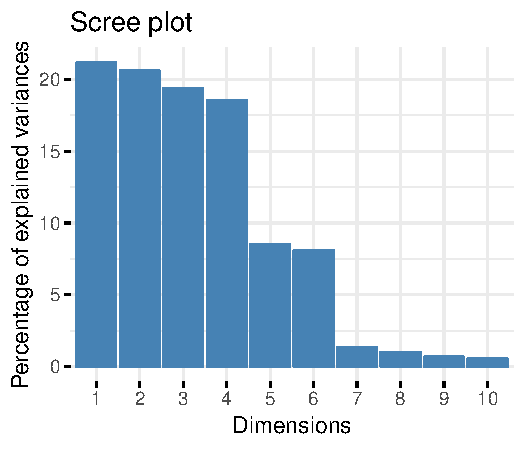
\includegraphics[width=\textwidth]{rock_scree2.pdf} 
        \caption{Rock}
    \end{subfigure} \\
    \begin{subfigure}[b]{0.5\textwidth}
        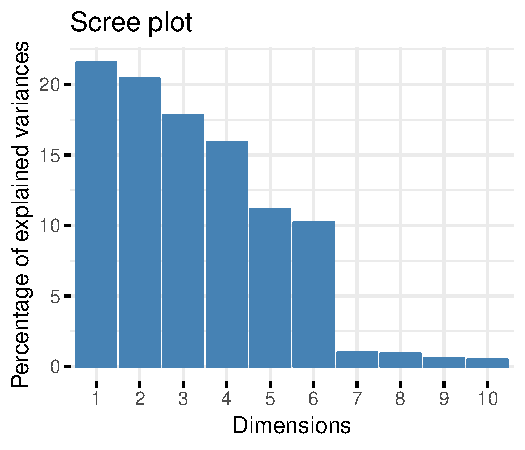
\includegraphics[width=\textwidth]{folk_scree2.pdf} 
        \caption{Folk}
    \end{subfigure}%
    \begin{subfigure}[b]{0.5\textwidth}
        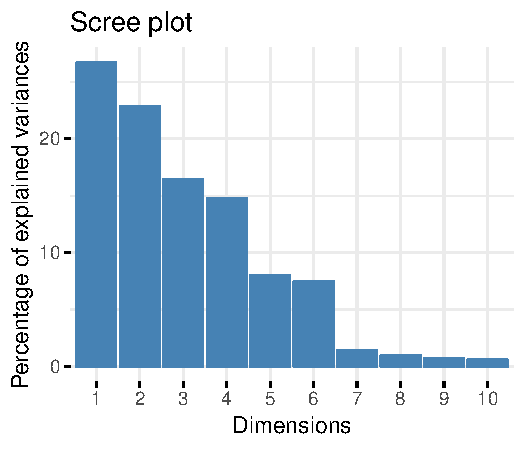
\includegraphics[width=\textwidth]{elec_scree2.pdf} 
        \caption{Electronic}
    \end{subfigure}%
\caption{Scree Plots (10 most significant PC's) by genre, means only}
\label{fig:scree2}
\end{figure}

This situation pushed us to try again PCA on different data matrices, where chroma features have been discarded and only means have undergone the same rows-and-columns normalization pre-treatment the previous data had been subjected to. The new results brought us to a considerably better situation, represented by scree plots in figure \ref{fig:scree2}. All these plots indicate -- more or less clearly -- a possibly optimal number of principal components equal to six.

\begin{figure}[h!]
\centering  
\begin{subfigure}[b]{0.5\textwidth}
        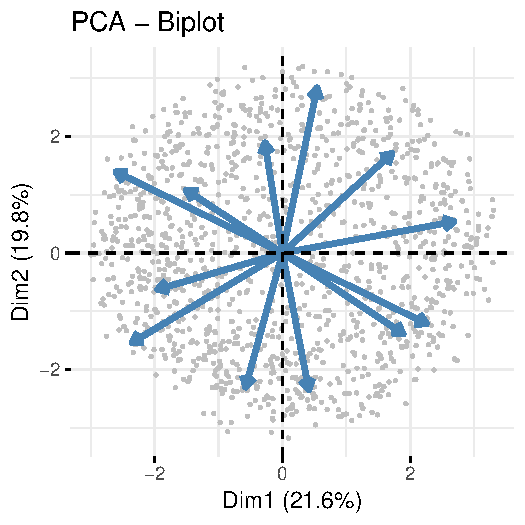
\includegraphics[width=\textwidth]{class_bipl.pdf} 
        \caption{Classical}
    \end{subfigure}%
    \begin{subfigure}[b]{0.5\textwidth}
        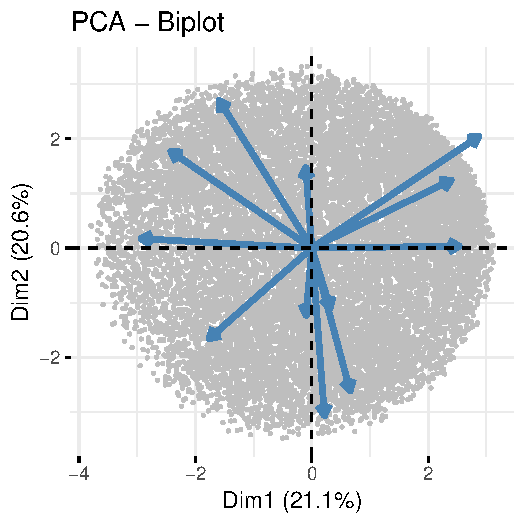
\includegraphics[width=\textwidth]{rock_bipl.pdf} 
        \caption{Rock}
    \end{subfigure} \\
    \begin{subfigure}[b]{0.5\textwidth}
        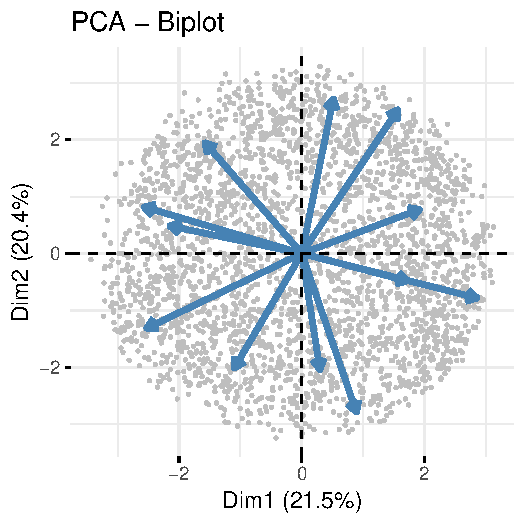
\includegraphics[width=\textwidth]{folk_bipl.pdf} 
        \caption{Folk}
    \end{subfigure}%
    \begin{subfigure}[b]{0.5\textwidth}
        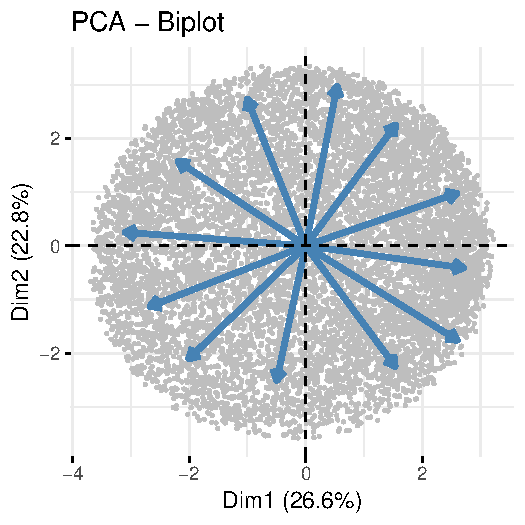
\includegraphics[width=\textwidth]{elec_bipl.pdf} 
        \caption{Electronic}
    \end{subfigure}%
\caption{BiPlots (2 most significant PC's) by genre, means only}
\label{fig:biplots}
\end{figure}

Extremely similar biplots (scatter plots showing points' coordinates in term of the two most representative principal components) generated through PCA on means and skewnesses together gave way to much more different ones when only means were considered, as shown in figure \ref{fig:biplots}.


These plots show exactly what we were unsure that could happen in terms of pitches (and, consequently, chroma features expression): a quick look at these graphs and at the pronounced differences among genres shown by the principal component loadings suggests that a genre can differentiate itself from other genres by the choices its artists make from the point of view of the pitches they want to use in their songs or, more broadly, the specific combinations of notes across the musical scale that they are more inclined to insert in the tracks they propose to listeners.

%\newpage
\section[Supervised Learning]{\textsc{Supervised Learning}}
In this part of our work we address the challenge of determining the genre of a track just by looking at its measurable characteristics, specifically the timbre. Such a task is non-trivial due to the wide diversity between the songs, even within the same category; moreover, crossovers and cross-genre songs not only exist, but are also very common. Notwithstanding these difficulties, each genre usually comes with a set of typical instruments, which make its sound unique and very recognizable by human listeners. In order to simplify the problem, we decided to consider only four out of the myriad of existing genres, carefully chosen to be both popular and sufficiently distinguishable with respect to each other.
Taking into account all these factors, our picks are hence the following: rock, folk, electronic and hip-hop music.

We tried to approach the problem with two different kinds of statistical techniques. On the one hand we have discriminant analysis (\emph{LDA}, \emph{QDA}), which attempts to identify the function that best separates the different classes of objects. On the other hand are non-parametric methods, like \emph{k-nearest neighbors}, which instead exploit local properties of the data to make predictions. As we will see, both strategy are valid and produce interesting results. 

\subsection{Discriminant analysis}

The objective of \emph{discriminant analysis} is to develop functions that are able to discriminate between the categories of the dependent variables in the best possible way. Such functions are particular combinations of the inputs: linear in the case of LDA, quadratic for QDA.
Instead of directly estimating the probability that an observation $x$ produces a response belonging to the $k$-th class, that is $\Pr(Y=k|X=x)$, discriminant analysis does the opposite: first, it produces a model for the \emph{density functions} $f_k(x) = \Pr(X=x | Y=k)$, then exploits the Bayes' theorem to flip the two events:
\begin{equation*}
    \Pr(Y=k|X=x) = \frac{\pi_k f_k(x)}{\sum_{i=1}^N \pi_i f_i(x)}
\end{equation*}
The values $\pi_i$ are the probabilities that a random sample belongs to class $i$, and can be easily obtained by observing the proportions in the training set. The form of $f_k(x)$ is unknown a priori; in most cases, including LDA and QDA, they are assumed to be Gaussian functions.\\

\noindent\textbf{Linear Discriminant Analysis}

In LDA, the distribution is Gaussian with mean $\mu_k$ and covariance matrix $\Sigma$. \\
In particular, the latter is common to all classes $k$.
\begin{equation*}
    f_k(x) = \frac{1}{\sqrt{(2\pi)^p |\Sigma|}}\exp{\left(-\frac{1}{2}{\left(x-\mu_k\right)}’\Sigma^{-1}\left(x-\mu_k\right)\right)}
\end{equation*}

If the density functions have such form, it is possible to prove that, the most-likely category $k^*$ for a given sample $x$ is the one that maximizes the quantity $\hat{\delta}_k$:

\begin{align*}
    &k^* = \argmax_k{\hat{\delta}_k}\\
    &\hat{\delta}_k(x) = x’ \hat{\Sigma}^{-1} \hat{\mu}_k - \dfrac{1}{2}\hat{\mu}_k’ \hat{\Sigma}^{-1} \hat{\mu}_k + \log{\hat{\pi}_k}
\end{align*}

After filtering the FMA dataset to keep only the songs belonging to the aforementioned genres, we performed LDA using the 19 timbre features as predictors.
The result is shown in Table \ref{table:ldaconfusion}; by summing all the diagonal elements of the confusion matrix, we could compute the overall prediction accuracy, which eventually turned out to be $67.4\%$.

\begin{table*}[h]
\centering
\begin{tabular}{|c|c|c|c|c|}
    \hline
                & Electronic & Folk & Hip-Hop & Rock \\ \hline
    Electronic  &   6776    &  367  &  338  &  1891 \\ \hline
    Folk        &   773     &  949  &  81   &  1000 \\ \hline
    Hip-Hop     &   1510    &  110  &  841  &  1091 \\ \hline
    Rock        &   1853    &  486  &  229  &  11591 \\ \hline
\end{tabular}
\caption{Confusion matrix produced by LDA, true values on rows}
\label{table:ldaconfusion}
\end{table*}

\noindent\textbf{Quadratic Discriminant Analysis}

Quadratic discriminant analysis is relatively similar to the linear one, with one major difference: unlike LDA, in QDA the covariance matrix is no longer shared between all the classes, but each category has its own $\Sigma_k$.
Under this assumption, the quantity to maximize becomes:
\begin{equation*}
    \hat{\delta}_k(x) = x’ \hat{\Sigma}^{-1}_k \hat{\mu}_k -\dfrac{1}{2} (x - \hat{\mu}_k)’ \hat{\Sigma}^{-1}_k (x-\hat{\mu}_k) -\dfrac{1}{2}\log \left|\hat{\Sigma}_k\right|+ \log{\hat{\pi}_k}.
\end{equation*}

Despite the increased flexibility in the QDA model with respect to LDA, the prediction improvement is negligible in our specific case. 
In fact, QDA was able to correctly predict the genre in $67.5\%$ of the cases, slightly more than LDA.

\begin{table*}[h]
\centering
\begin{tabular}{|c|c|c|c|c|}
    \hline
                & Electronic & Folk & Hip-Hop & Rock \\ \hline
    Electronic  &   6799    &  628  &  528  &  1417 \\ \hline
    Folk        &   590     &  1452 &  110  &  651  \\ \hline
    Hip-Hop     &   1272    &  223  &  1201 &  856  \\ \hline
    Rock        &   2114    &  827  &  362  &  10856 \\ \hline
\end{tabular}
\caption{Confusion matrix produced by QDA, true values on rows}
\label{table:qdaconfusion}
\end{table*}

In both experiments we adopted LOOCV cross-validation to avoid overfitting, which is anyway unlikely due to the large number of samples with respect to the amount of parameters to fit. Similarly, we also tried with k-fold with $k=10$, yet without noticing any relevant difference.

The comparison of LDA and QDA results suggests that the genre classes are approximately linearly separable in the domain of timbre features, therefore increasing the classifier order does not provide significant benefits.

\subsection{Local methods}

The other approach is radically different and consists in using local information of the dataset to predict the response of a particular sample. In our analysis we considered \emph{k-nearest neighbors}, probably the most popular among these methods.\\

\noindent\textbf{k-nearest neighbors}

The k-NN classifier follows a very simple rule: the predicted response for a given sample corresponds to the most common one among its $k$ closest elements. Actually, a proper definition of the methods must also specify how the distance is calculated between two elements, and there exist several options.
Our choice fell on the $L^2$ distance (\emph{Euclidean)}, defined as follows:
\begin{equation*}
    dist(x, y) = ||x - y||_2 = \sqrt{\sum_{i=1}^p (x_i-y_i)^2}
\end{equation*}

In general, the number $k$ affects the behaviour of the algorithm: small values cause the prediction to be greatly affected by local characteristics: this is not necessarily a good choice, since a larger flexibility also means that the model is more subject to local fluctuations.

\begin{figure}[ht]
    \centering
        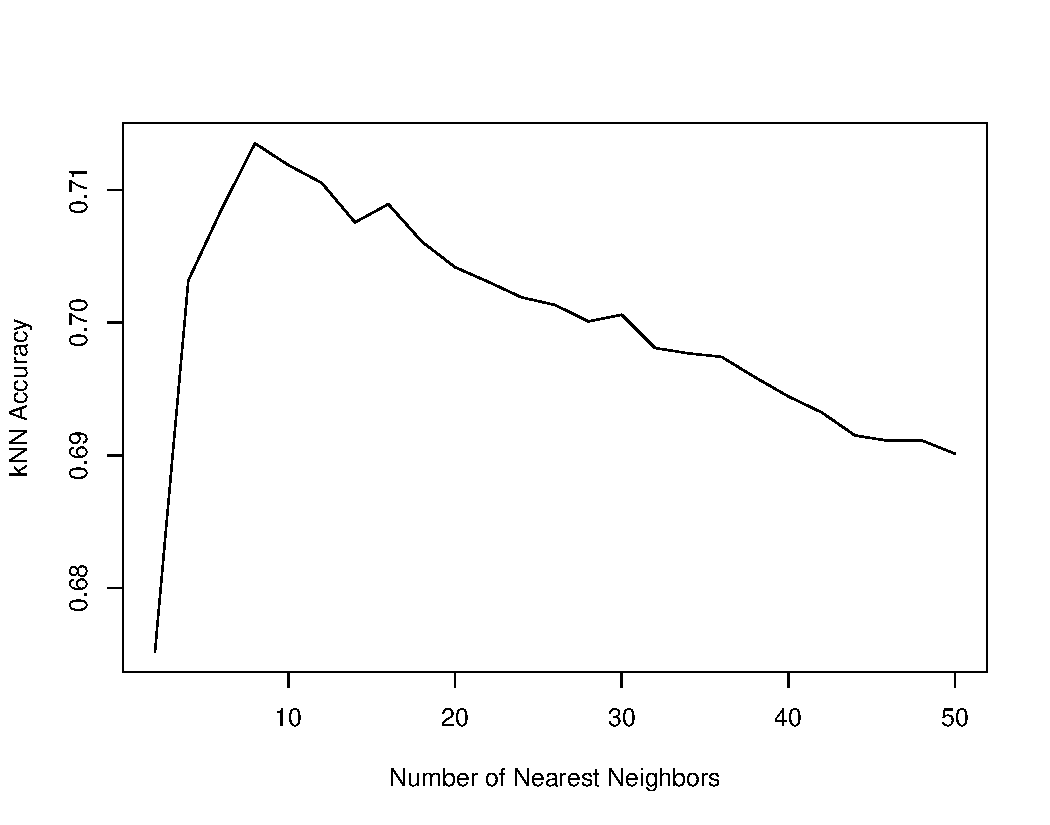
\includegraphics[width=\linewidth]{keynn.pdf}
        \caption{k-nearest neighbors accuracy as function of k}
        \label{fig:knn}
\end{figure}

From our experiments, it turns out that kNN outperforms both LDA and QDA, being able to reach at most a $71.2\%$ accuracy with $k=8$.\\
The corresponding confusion matrix is displayed in Table \ref{table:knnconfusion}. 
Figure \ref{fig:knn} shows how the overall performance strongly depends on the selection of $k$: for instance, switching from $k=2$ to $k=4$ is enough to produce a $3\%$ boost in the accuracy, and it keeps increasing up to $k=8$, then starts to slowly drop for $k>8$.

\begin{table*}[ht]
\centering
\begin{tabular}{|c|c|c|c|c|}
    \hline
                & Electronic & Folk & Hip-Hop & Rock \\ \hline
    Electronic  &   6845    &  418  &  545  &  1564 \\ \hline
    Folk        &   648     &  1376 &  127  &  652  \\ \hline
    Hip-Hop     &   1462    &  113  &  1119 &  858  \\ \hline
    Rock        &   1753    &  397  &  337  &  11672 \\ \hline
\end{tabular}
\caption{Confusion matrix produced by 8-NN, true values on rows}
\label{table:knnconfusion}
\end{table*}

\newpage

\section[Conclusions]{\textsc{Conclusions}}
Machine learning applied to musical analysis is a rapidly-expanding field, which spans a broad range of different application, not only limited to genre/artist recognition: from detection of harmonic patterns in songs and their occurrence in the music of different composers and their genres-specific distribution, to the development of ever more accurate algorithms for the prediction of user preferences by streaming platforms, machine-based music generation and optimization of musical composition. 

As regards to our analysis, the results we obtained were satisfyingly surprising: as previously discussed, the unsupervised analysis results estimates showed simple but clear regularities across genres, while the supervised analysis techniques we used to classify tracks by genres showed that the most effective procedures were also the simplest ones (although by a small margin). 

However, the main limitation we encountered during our analysis has been represented by the deficiency of informative labels provided by the meta-dataset. Most ironically, while our main dataset was made up of an higher number of sound features than we were able to deal with, its coupled meta-dataset was missing important pieces of information.
Available meta-labels consisted of track title, genre, performer, plus a set of features summarizing the career of the artist. 
It is immediately clear the lack of many sound-related information, such as tonality, number and type of instruments played. 

Although this kind of data may appear redundant as already encoded in the main dataset (i.e. chroma and timber features), the presence of categorical labels would have been useful as a resource to validate the selection of different subsets of features depending on what goals our analysis was aiming at. Furthermore, it would have allowed a meaningful interpretation of the outcomes of unsupervised analysis from a musical point of view.
Another kind of missing information is represented by track labels - such as sub-genre - which could have been employed as additional classifiers to refine our prediction algorithm.

Consistent with this view, clustering analysis performed upon classical-labelled observations provides a paradigmatic example. As previously described, our feature selection was led by the assumption that most of the variability between songs belonging to the same class can be accounted for by the choice of different tonalities rather than the use of different instruments. This reasonable postulate allowed us to obtain stable results, consistent among genres - even in the classical subset -. However, in the latter case is likewise reasonable to assume that significant differences can be spotted by timber features, as the tracks differ not only in the type of instrument played (e.g. string or percussion instruments), but also in their number (e.g. symphonic versus chamber orchestra).

Given that, collection of missing metadata information represents a necessary step, which is an urgent as much as a challenging one. Although, once performed it would enable us to look at the data from new, unexplored perspectives -- otherwise inaccessible.
\newpage

\appendix
\section[Snippets of Code]{\textsc{Snippets of Code}}

Our analyses were performed entirely on R. We used standard libraries for most of the work we wanted to do, but we had the possibility to take great advantage of packages designed specifically to produce clearer and aesthetically more pleasant representations than those offered as standard by basic libraries. These packages will always be evoked in the code when needed.

\subsection{Unsupervised Techniques}
Since we run the same lines of code for 4 different data matrices, we we'll report them only once for the sake of clarity.

\vspace{1cm}

\noindent\textbf{Cluster Analysis}
\begin{lstlisting}
#this allows to obtain all the representations reported in this work
library(factoextra)

#allows for silhouette width computation
library(cluster)

#this command normalizes rows and columns of the data matrix genrex
norm_genrex <- scale(t(scale(t(genrex),center = TRUE, scale = TRUE)), center = TRUE, scale = TRUE)

#elbow plot generator with hierarchical clustering (euclidean distance and complete linkage)
elbowplot <- fviz_nbclust(norm_genrex, FUNcluster = hcut, hc_method = "complete", method = "wss", diss = NULL, k.max = 10, print.summary = TRUE)

#clusterizes the observations in norm_genrex into k clusters through k-means clustering by using centroids obtained by hierarchical clustering
genrex_clust <- hkmeans(norm_genrex, k, hc.metric = "euclidean", hc.method = "complete", iter.max = 10, km.algorithm = "Hartigan-Wong")

#draws a colorized dendrogram like those seen in section 3.1. Computationally very expensive (we don't know the reason of this so we suggest to use it wisely, the rock-related dendrogram took two hours to draw with a desktop workstation!)
dendrogram <- fviz_dend(genrex_clust, show_labels=FALSE)

#silhouette plot generator for the outcome genrex_clust
silplot <- fviz_silhouette(silhouette(genrex_clust$cluster, dist(norm_genrex)))
\end{lstlisting}

\vspace{1cm}

\noindent\textbf{Principal Component Analysis}

\begin{lstlisting}
#stats package is mandatory for PCA
library(factoextra, cluster, stats)

#performs PCA
genrex_pca <- prcomp(norm_genrex, retx = TRUE, center = TRUE, scale. = TRUE, tol = NULL, rank. = NULL)

#draws a screeplot using data generated by the previous command
fviz_eig(genrex_pca, choice = "variance", geom = "bar")

#useful to drop columns from matrices
library(dplyr)

#performs row and column standardization on a matrix where only the first 12 features have been kept (the chroma feature means in our case)
norm_meansx <- scale(t(scale(t(genrex[,1:12]),center = TRUE, scale = TRUE)), center = TRUE, scale = TRUE)

#as before
meansx_pca <- prcomp(norm_meansx, retx = TRUE, center = TRUE, scale. = TRUE, tol = NULL, rank. = NULL)
fviz_eig(meansx_pca, choice = "variance", geom = "bar")

#biplot generator
fviz_pca_biplot(class_avgpca, axes = c(1, 2), geom.ind = "point", geom.var = "arrow", col.ind = "grey", fill.ind = "white", col.var = "steelblue", fill.var = "white", gradient.cols = NULL, label = "all", invisible = "none", repel = FALSE, habillage = "none", palette = NULL, addEllipses = FALSE, title = "PCA - Biplot", pointsize=0.3, arrowsize=1.3)
\end{lstlisting}

\vspace{0.7cm}

\subsection{Supervised Techniques}

\vspace{0.5cm}

\noindent\textbf{LDA and QDA}
\begin{lstlisting}
library(class, dplyr, mass)

#data matrix (the first column indicates the genre)
allgenres

#standardizing rows (considering obviously only the continuous features)
norm_meansx <- cbind(allgenres[,1], t(scale(t(allgenres[,2:21]),center = TRUE, scale = TRUE)))

#performs LDA with LOOCV, Vn is the name of the nth column in the matrix (V1 indicates the genre)
allg_lindisc <- lda(V1~V2+V3+V4+V5+V6+V7+V8+V9+V10+V11+V12+V13+V14+V15+V16+V17+V18+V19+V20, norm_meansx, CV=T)

#creates a table aggregating observations by genre predicted by LDA and actual genre
linda_tab <- table(norm_meansx$V1, allg_lindisc$class)

#estimates the out-of-sample success rate (since we are dealing with LOOCV)
sum(linda_tab[row(linda_tab)==col(linda_tab)])/sum(linda_tab)

#same as before but with QDA
allg_qudisc <- qda(V1~V2+V3+V4+V5+V6+V7+V8+V9+V10+V11+V12+V13+V14+V15+V16+V17+V18+V19+V20, norm_meansx, CV=T)
quda_tab <- table(norm_meansx$V1, allg_qudisc$class)
sum(quda_tab[row(quda_tab)==col(quda_tab)])/sum(quda_tab)
\end{lstlisting}

\vspace{1cm}

\noindent\textbf{kNN}
\begin{lstlisting}
#kNN classification using all the points in the dataset except for the one that needs to be classified (sort of LOOCV). Classification using i nearest neighbors (to be specified)
nearest.neigh <- knn.cv(select(norm_meansx, -c(V1)),factor(norm_meansx[,1]) , k = i, l = 0, prob = FALSE, use.all = TRUE)

#same as the previous code snippet
nntab <- table(norm_meansx$V1, nearest.neigh)
sum(nntab[row(nntab)==col(nntab)])/sum(nntab)
\end{lstlisting}
\nocite{*}
\newpage
\bibliographystyle{plain}
\bibliography{references}
\end{document}